%!TEX program = xelatex.exe
\documentclass[14pt,a4paper]{article}
% \usepackage[pdftex,
%     pdfauthor={К.С.~Пилипенко},
%     pdfsubject={The Subject},
%     pdfkeywords={Первое ключевое слово, второе ключевое слово},
%     pdfproducer={LuaLatex with hyperref},
%     pdfcreator={Lualatex},
%     % hidelinks
% ]{hyperref}
%%%%%%%%%%%%%%Пользовательские команды%%%%%%%%%
\usepackage{calc}
\usepackage{color}
\usepackage{listing}
\usepackage{svg}
\usepackage{hhline}
\usepackage{multirow}
\usepackage{latexsym,amsmath,amssymb,amsbsy,graphicx}
\usepackage{listings}
\usepackage{icomma}
\usepackage[obeyspaces]{url} %Позволяет прописывать путь к файлам
\usepackage[american,siunitx]{circuitikz}
\def\centerarc[#1][#2](#3:#4:#5){\draw[#1]($(#2)+({#5*cos(#3)},{#5*sin(#3)})$)}
\usepackage[version=4]{mhchem} % the canonical chemistry package (example: \ce{^{32}_{15}P})
\usepackage{graphicx}
\usepackage{pgfplots}
\usepackage{wrapfig}
\graphicspath{{images/}}
\DeclareGraphicsExtensions{.pdf,.png,.jpg}
\usepackage{hyperref}
\hypersetup{
    colorlinks=true,
    linkcolor=blue,
    filecolor=magenta,      
    urlcolor=cyan,
    pdfauthor={К.С.~Пилипенко},
    pdfsubject={Основы обработки результатов исследования в физике},
    % pdfkeywords={Первое ключевое слово, второе ключевое слово},
    pdfproducer={LuaLatex with hyperref},
    pdfcreator={Lualatex},
    pdfpagemode=FullScreen,
    }
\urlstyle{same}
%Форматирование разделов
\usepackage{titlesec}
\usepackage{multicol} %Многоколоночный список
%%% Кастомизация разделов
\titleformat
{\section} % command
[block] % shape
{\normalfont\bfseries\itshape} % format
{Задание №\thesection.}{0.5em}{} % label
\newcommand{\progress}{\begin{center}\large\bfseries Ход работы\end{center}}
\newcommand{\questions}{\begin{center}\large\bfseries  Контрольные вопросы \end{center}}
%%%%%%%%%%%%%%%%%%%%%%%%Оформление по ГОСТУ
\usepackage{fontspec}
\setmainfont[Renderer=Basic,Ligatures={TeX}]{Times New Roman}
% \usepackage[english,russian]{babel} %Поддержка русской локализации
\setmonofont{dejavusansmono} % verbatim с кириллицей
\usepackage[14pt]{extsizes} % для того чтобы задать нестандартный 14-ый размер шрифта
\usepackage{indentfirst} %Задаёт отступ самого первого абзаца
\setlength\parindent{1.25cm}
\usepackage[a4paper, left=3cm, top=1.5cm, right=1.5cm, bottom=2cm]{geometry}
\usepackage{setspace}
\sloppy %Выравнивание текст по ширине и решение проблемы переполнением строки
\onehalfspacing %Полуторный интервал
%%%%%%%%%%%%%%%%%%%%%%%%%%%%% Добавление списка литературы
\usepackage{polyglossia}[2014/05/21]            % Поддержка многоязычности (fontspec подгружается автоматически)
\setmainlanguage[babelshorthands=true]{russian}  % Язык по-умолчанию русский с поддержкой приятных команд пакета babel
\setotherlanguage{english}                       % Дополнительный язык = английский (в американской вариации по-умолчанию)
\setmonofont{Courier New}
\newfontfamily\cyrillicfonttt{Courier New}
    \defaultfontfeatures{Ligatures=TeX,Mapping=tex-text}
\setmainfont{Times New Roman}
\newfontfamily\cyrillicfont{Times New Roman}
\setsansfont{Arial}
\newfontfamily\cyrillicfontsf{Arial}
\usepackage[
    bibencoding=utf8,% кодировка bib файла
    sorting=none,% настройка сортировки списка литературы
    style=gost-numeric,% стиль цитирования и библиографии (по ГОСТ)
    language=autobib,% получение языка из babel/polyglossia, default: autobib % если ставить autocite или auto, то цитаты в тексте с указанием страницы, получат указание страницы на языке оригинала
    autolang=other,% многоязычная библиография
    clearlang=true,% внутренний сброс поля language, если он совпадает с языком из babel/polyglossia
    defernumbers=true,% нумерация проставляется после двух компиляций, зато позволяет выцеплять библиографию по ключевым словам и нумеровать не из большего списка
    sortcites=true,% сортировать номера затекстовых ссылок при цитировании (если в квадратных скобках несколько ссылок, то отображаться будут отсортированно, а не абы как)
    doi=false,% Показывать или нет ссылки на DOI
    isbn=false,% Показывать или нет ISBN
]{biblatex}
\DeclareSourcemap{ %модификация bib файла перед тем, как им займётся biblatex 
    \maps{
        \map{% перекидываем значения полей language в поля langid, которыми пользуется biblatex
            \step[fieldsource=language, fieldset=langid, origfieldval, final]
            \step[fieldset=language, null]
        }
    }
}
\emergencystretch=1em
\addbibresource{literature.bib}
%%%%%%%%%%%%%%%%%%%%%%%%
\author{\href{mailto:www-kirill.pilipenko@yandex.ru}{К.С.~Пилипенко} \href{https://github.com/PilipenkoKirill/MeasurementLabs}{
\includegraphics[width=.5cm]{images/gitHubLogo.pdf}}} %Через \and можно добавить ещё авторов
\date{\the\year{}}

\title{Лабораторная работа №5.1 \\ \textit{Построение графиков в программе SciDAVis}}
\begin{document}
\maketitle
Не смотря на то, что Excel успешно справляется с большинством задач анализа и визуализации данных он используется в первую очередь для предварительной обработки данных. Для построение красивых графиков используются другие программы, такие как: \href{https://www.originlab.com/index.aspx?go=Products/Origin}{Origin и OriginPro}, \href{https://www.python.org/}{Python} + библиотеки matplotlib+numpy+scipy (самый продвинутый и гибкий набор инструментов!), \href{https://scidavis.sourceforge.net/}{SciDAVis}, \href{https://www.ctan.org/pkg/pgfplots}{pgfplots} (пакет \LaTeX, который используется в данном сборнике лабораторных работ), Gnuplot, LabPlot, Grace QtiPlot и др. Origin\footnote{С инструкцией по установке OriginPro можно ознакомиться в приложении} является наиболее универсальной и многофункциональной программой, при этом является платной. Python с подключенными библиотеками предлагает самый продвинутый и гибкий набор инструментов, но при этом он сложен для новичков и управление осуществляется без \href{https://ru.wikipedia.org/wiki/%D0%93%D1%80%D0%B0%D1%84%D0%B8%D1%87%D0%B5%D1%81%D0%BA%D0%B8%D0%B9_%D0%B8%D0%BD%D1%82%D0%B5%D1%80%D1%84%D0%B5%D0%B9%D1%81_%D0%BF%D0%BE%D0%BB%D1%8C%D0%B7%D0%BE%D0%B2%D0%B0%D1%82%D0%B5%D0%BB%D1%8F}{GUI}.

В силу изложенного предлагается остановиться на программе SciDAVis. SciDAVis~---~это бесплатное и свободное программное обеспечение, которое предлагает пользователю дружелюбный и интуитивно понятный интерфейс. 

\begin{center}
    \textbf{Ход работы:}
\end{center}
\section{Установка программы и знакомство с интерфейсом}
\begin{enumerate}
    \item Скачайте по \href{https://sourceforge.net/projects/scidavis/files/latest/download}{ссылке} программу;
    \item Установите программу следуя рекомендациям установщика.
\end{enumerate}
% \section{Оцифровка графиков}
% \begin{enumerate}
%     \item После установки и запуска программы откройте специальный инструмент OriginPro для оцифровки графиков (tools$\rightarrow$Digitizer). Импортируёте изображение. \\
%     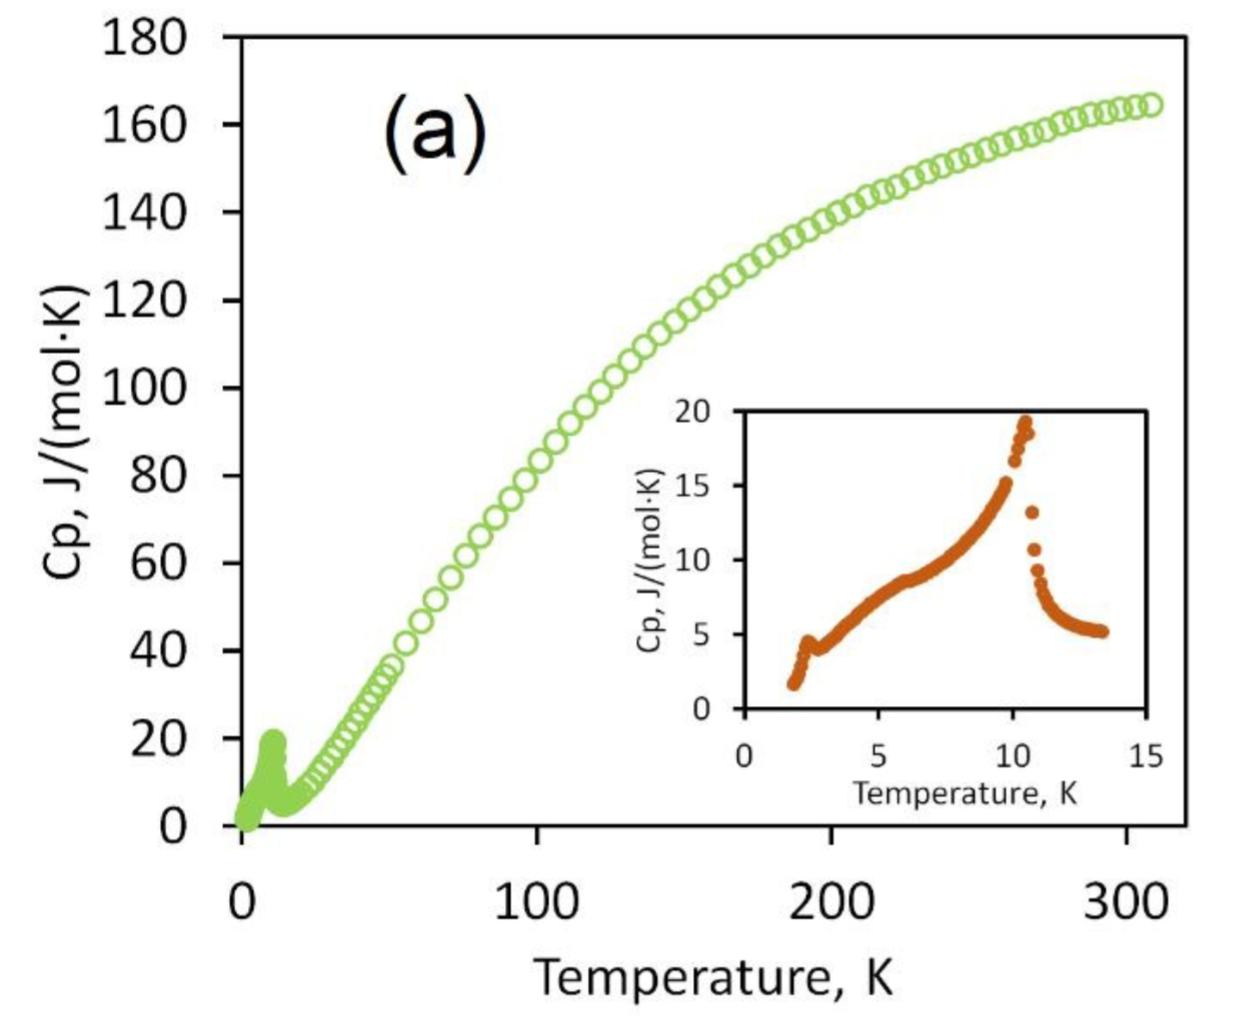
\includegraphics[width=.7\textwidth]{HeatCapExm.png} 
%     \item Регулируйте положение линий, чтобы они соответствовали определённым значениям на осях рисунка. Укажите якорные значения в колонке Axis Value \\
%     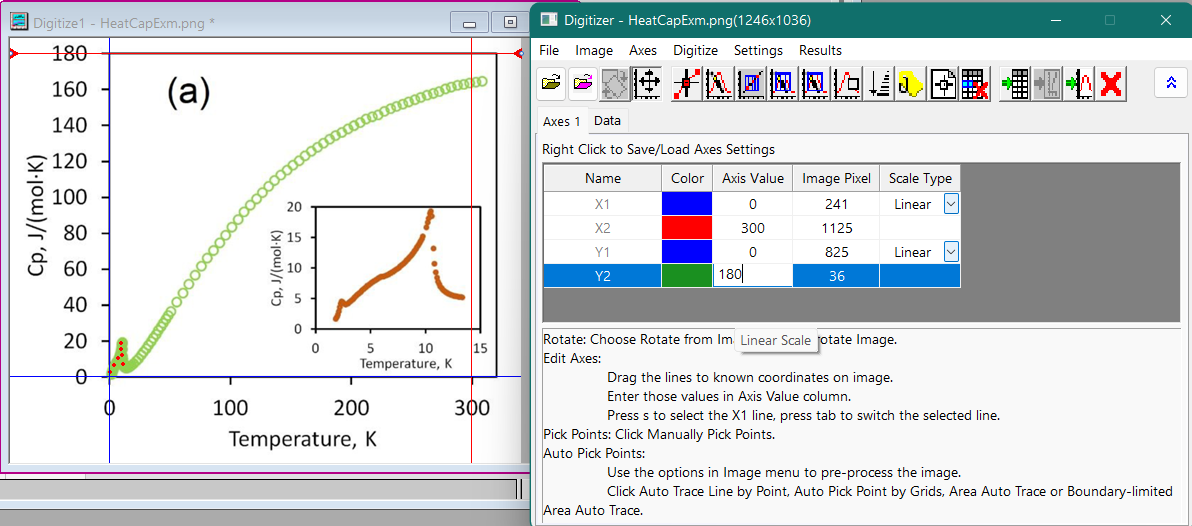
\includegraphics[width=.7\textwidth]{HeatCapExmDragLines.png} 
%     \item Выберете ручной (Manually Pick Points) или автоматический (Auto Pick Points) способ задания точек. Оцифруйте все точки на большом графике.
%     \item После этого нажмите на кнопку Go to Data в окне Digitizer и экспортируйте таблицу в формат Excel (В главном окне File$\rightarrow$Export$\rightarrow$Excel). Желательно использовать формат .xslx
% \end{enumerate}   
\section{Построение графиков}
\begin{enumerate}
    \item Используя данные из предыдущей лабораторной работы (№5) составьте график. 
    \item Дайте названия осей в формате: \verb|{физ. вел.}, {ед. изм.}|, например x -- сила тока в амперах, а y -- мощность в ваттах, или можете придумать названия осей сами, вспомнив другие квадратичные зависимости в физике. Далее расположите названия осей по центру числовой шкалы. Параметры шрифта по возможности должны быть такими же, как и в предполагаемом документе, где будет находится график: кегль -- 14 пт, семейство -- Roman);
    \item Проведите линейную регрессию для точек выборки;
    \item Задайте относительную погрешность 5\% для оси Y;
    \item Оформите легенду, добавив название <<Экспериментальные точки>> для точек выборки, а для аппроксимирующей линии укажите формулу и параметры аппроксимации с правильно округлёнными погрешностями (можно получить из консоли, где появляется информация после добавления линейной регрессии);
    \item Цветовую палитру можете выбрать любую, главное чтобы цвета хорошо контрастировали с фоном;
    \item Экспортировать рисунок в векторном формате, например в \verb|.svg|.
\end{enumerate}

% \textbf{Контрольные вопросы} \\
% \begin{enumerate}
%     \item 
% \end{enumerate}
% \textbf{Методические рекомендации к заданию для обучающихся:} 

Выполнение практического задания проводится обучающимся
самостоятельно. Для расчетов используются результаты собственных
исследований полученных в ходе выполнения лабораторных работ по курсу <<механика>> (РЕКОМЕНДУЕТСЯ)
% , при отсутствии необходимого материала данные предоставляются преподавателем по запросу студента
. 
Работа выполняется в программе \href{https://mega.nz/folder/0EUyAKgC#4X5RubnYkoUUJYhwDDpKbg}{Microsoft Office Excel} или \href{https://www.libreoffice.org/download/download-libreoffice/?type=win-x86_64&version=7.4.0&lang=ru-RU}{LibreOffice Calc}. Результаты выполнения задания оформляются в файле с расширением ".xlsx". В названии файла укажите свою фамилию с инициалами, курс и группу.
% \section{Рекомендуемая литература}
% \begin{enumerate}
%     \item \url{https://www.google.com/url?sa=t&rct=j&q=&esrc=s&source=web&cd=&cad=rja&uact=8&ved=2ahUKEwiLuJmd6-L6AhWrk4sKHZoBCE0QFnoECCUQAQ&url=https%3A%2F%2Foit.colorado.edu%2Fsites%2Fdefault%2Ffiles%2FOrigin2016_UserGuide.pdf.pdf&usg=AOvVaw1_NeiHINEkOymJnRjABlx8}
% \end{enumerate}

\begin{center}
	\textbf{\Large Приложение}
\end{center}
Инструкция к установке программы OriginPro
\begin{enumerate}
    \item Скачайте по \href{https://mega.nz/folder/4R9xHYgT#LjgmYjooWK4WEsR4ylHn_w}{ссылке} программу;
    \item Установить программу в режиме OriginPro Trial следуя правилам установщика; 
    \item Заменить файлами из папки \path{Crack\Fix3} (\verb=ok.dll= и \verb=ou.dll=) соответствующие файлы в папке с установленной программой (стандартный путь: \path{c:\Program Files\OriginLab\Origin2021\}, который у вас может отличаться).
\end{enumerate}
\end{document}